\documentclass[a4paper, 9pt, draft]{amsart}
\usepackage[english]{babel}
\usepackage{amsmath}
\usepackage{amssymb}
\usepackage{amsfonts}
\usepackage{mathtools}
\usepackage{diagbox}
\usepackage{booktabs}
\usepackage{enumitem}
\usepackage{color}
\usepackage{hyperref}
\usepackage{tikz}
\usepackage{accents}
\usepackage{standalone}
\usepackage{bm}
\usepackage{multicol}
\usepackage{stmaryrd}
\usepackage{graphicx}
\usepackage{float}
\usepackage{syntax}
\usepackage[final]{listings}
\usepackage[font={small,sc}]{caption}

\usetikzlibrary{fit}
\usetikzlibrary{backgrounds}
\usetikzlibrary{positioning}
\usetikzlibrary{decorations}
\usetikzlibrary{decorations.pathmorphing}
\usetikzlibrary{arrows.meta}
\usetikzlibrary{chains}
\usetikzlibrary{shapes.multipart}
\usetikzlibrary{scopes}
\usetikzlibrary{arrows}


\hyphenation{block-chain block-chains}
\hyphenation{crypto-graphically}

\hypersetup{colorlinks,
    citecolor=black,
    filecolor=black,
    linkcolor=black,
    urlcolor=blue,
    pdftex}

\setlist[description]{leftmargin=1.2cm, labelindent=\parindent}
\setlist[enumerate]{leftmargin=1.2cm, labelindent=\parindent}

\newcommand*\eg{e.g.\ }
\newcommand*\ie{i.e.\ }

\title[Radicle]{Radicle}
\author{Monadic}
\date{2018}

\newcommand{\oscoin}{\textsc{\small{oscoin}}}
\newcommand{\blake}{\textsc{\small{blake2}}}
\newcommand{\hash}{\mathsc{hash}}
\newcommand{\coin}{$\Theta$}
\newcommand{\mathsc}[1]{\text{\normalfont\scshape#1}}
\newcommand{\tx}[2]{\langle \mathsc{#1}, #2 \rangle}
\newcommand{\tuple}[1]{\langle #1 \rangle}
\newcommand{\cvdots}{\multicolumn{1}{c}{\small{\vdots}}}
\newcommand{\dep}{\xrightharpoondown[e]{d}}
\newcommand{\notice}[1]{{\color{red}#1}}
\newcommand{\comment}[1]{{\color{gray}#1}}
\newcommand{\todo}[1]{\comment{\noindent\texttt{\small\emph{TODO: #1}}}}

\newcommand{\rootchain}{\gamma}
\newcommand{\State}{\mathcal{S}}
\newcommand{\state}{\mathcal{S}}
\newcommand{\Ledger}{\mathcal{L}}
\newcommand{\ledger}{\mathcal{L}}
\newcommand{\Orgs}{\mathcal{O}}
\newcommand{\apply}{\Upsilon}
\newcommand{\fold}{\Upsilon}
\newcommand{\tree}{\mathcal{C}}
\newcommand{\op}{T}
\newcommand{\env}{\rho}
\newcommand{\cont}{\kappa}
\newcommand{\mem}{\sigma}
\newcommand{\val}{\epsilon}
\newcommand{\denotation}[2]{
    \ensuremath{\mathcal{E}_{#1} \llbracket #2 \rrbracket }}
\newcommand{\denotationdesc}[3]{
    \ensuremath{\mathcal{E}_{#1} \llbracket #2 \rrbracket \env \cont \mem &= #3  }}
\newcommand{\variable}{\nu}
\newcommand{\prog}{\pi}
\newcommand{\rad}{\textsc{Radicle} }
\newcommand{\lam}{\text{\texttt{lambda }}}
\newcommand{\define}{\text{\texttt{define}}}
\newcommand{\deref}{\text{\texttt{deref!}}}
\newcommand{\mkref}{\text{\texttt{ref!}}}
\newcommand{\set}{\text{\texttt{set!}}}
\newcommand{\quotem}{\text{\texttt{quote}}}
\newcommand{\evalm}{\text{\texttt{eval}}}
\newcommand{\ifm}{\text{\texttt{if}}}
\newcommand{\stdfn}[2]{
    \texttt{#1}
    #2
    }



\DeclareMathOperator{\eval}{\Xi}

% Adjust spacing around equations. It can be a bit tight!
\expandafter\def\expandafter\normalsize\expandafter{%
    \normalsize%
    \addtolength{\abovedisplayskip}{2pt}%
    \addtolength{\abovedisplayshortskip}{2pt}%
    \addtolength{\belowdisplayskip}{2pt}%
    \addtolength{\belowdisplayshortskip}{2pt}%
}%

\newenvironment{fig}
  {\par\bigskip\noindent\minipage{\linewidth}}
  {\endminipage\par\bigskip}

% No paragraph indentation after section headers.
\makeatletter
\let\@afterindenttrue\@afterindentfalse
\makeatother

% Issue amend operator.
\DeclareMathOperator{\amend}{\times}

\newenvironment{epigraph}[2][]
{\leftskip=1cm \def\epigraph@author{#2} \smallskip\itshape}
{\par\vspace{0.5em}\normalfont\hfill---\ \epigraph@author\hspace*{0.2cm}\par\medskip}
\makeatother

% Tikz stuff

\tikzstyle{block} = [rectangle, draw,
    text width=5em, text centered, rounded corners, minimum height=4em]
\tikzstyle{line} = [draw, -latex']

\setlength{\textwidth}{\paperwidth}
\addtolength{\textwidth}{-4cm}
\setlength{\textheight}{\paperheight}
\addtolength{\textheight}{-5cm}
\calclayout

\begin{document}
\begin{abstract}
    ...
\end{abstract}
\maketitle

\setlength{\columnsep}{20pt}
\begin{multicols}{2}

\section{Introduction}

\begin{epigraph}{The Open-Source Everything Manifesto}
    \noindent It is in this light that we must recognize that only a restoration of
    open-source culture, and all that enables across the full spectrum of
    open-source possibilities, can allow humanity to harness the distributed
    intelligence of the collective and create the equivalent of heaven on Earth
    -- in other words, a world that works for all.
\end{epigraph}

\noindent \oscoin{} is a protocol and token that attempts to provide a decentralized
hosting solution for open-source code with the means to collaborate on, govern
and fund open-source software projects sustainably, with no central authority
in control.

\subsection{Core Components}

\oscoin{} introduces a few components that, taken together, constitute the core
of the proposed solution.

\begin{description}
    \item[Registry] The registry, formally $\mathcal{R}$, is a
        decentralized service which provides a canonical record of projects and
        organizations known to the network.
    \item[Treasury] The treasury, formally $\mathcal{T}$, is a
        decentralized service with the purpose of funding open-source projects
        of value on the network.
    \item[Network] A decentralized code hosting network, formally
        $\mathcal{N}$, which hosts all the source code known to the network
        in a way that is available and censor-proof.
    \item[Dependency Graph] The dependency graph $\mathcal{D}$, is a global
        graph of all dependencies known to the network, whether these
        dependencies are hosted on the network or hosted externally.
    \item[Oscoin] The \oscoin{} token is a cryptographic token used for value
        exchange in the network.
\end{description}

\subsection{Protocol Overview}

\begin{itemize}
    \item The \oscoin{} network is a decentralized code hosting network
        composed of different kinds of participants, including
        \emph{maintainers}, \emph{contributors} and \emph{operators}.
    \item Maintainers and contributors collaborate around software projects
        organized in code repositories hosted by the network.
    \item Through the registry $\mathcal{R}$, participants discover, support
        and join open-source projects.
    \item Funds available for distribution are first sent to the treasury
        $\mathcal{T}$, before being distributed to chosen organizations.
    \item Token holders are able to pledge a certain amount of tokens towards
        an organization. This has the effect of signaling the treasury that a
        given organization has value to them, influencing the distribution of
        funds.
    \item Organizations are able to use the funds allocated to them for
        whichever purpose they see fit. \emph{Issues} and \emph{smart
        contracts} are used as a means for smart distribution of tokens from
        within an organization, to its constituent members.
    \item Code is attached to issues in the form of \emph{patches}. Issues act
        as the epicenter of change and collaboration around a project.
\end{itemize}
\pagebreak

\section{Language Syntax and Semantics}

\rad is a a Lisp dialect. It uses prefix parenthesized function application,
supports recursion, has first-class functions, is dynamically typed, and
homoiconic. It differs from most Lisps in a few aspects, described below.

Like most Lisps, binding is lexical. Unlike most Lisps, \rad has a
\textit{hyperstatic} global environment, meaning that the resolution of free
variables takes place at the definition site rather than call-site. Thus:

\begin{lstlisting}[language=Lisp, basicstyle=\small\ttfamily]
(define (foo) x) ;; error - "x" is not defined
(define x 3)
(foo) ;; 3
(define x 5)
(foo) ;; still 3
\end{lstlisting}

Usually \rad programs are an interleaving of code written by multiple people,
and each developer cannot in general be certain of what code will end up in the
program between the text that she knows about and her new submission. A
hyperstatic environment ameliorates the resulting unpredictability by making
function calls by default (i.e., modulo the usage of mutable references)
independent of intermediate submissions.

\rad does not have macros. Instead, it allows for a complete redefinition of
the intepreter via redefinitions of \texttt{eval}.

\begin{lstlisting}[basicstyle=\small\ttfamily]
(define (eval expr) 3) ;;
5 ;; --> 3
\end{lstlisting}

This enables users to very easily define sublanguages for new chains, or amend
the language running in the current one.

% TODO: maybe move to Related Work section
\subsection{Connection to Reflective Towers} The \texttt{eval}-redefinition
mechanism resembles prior work on \textit{reflective towers}. A reflective
tower is an infinite series of levels of interpreters, $L_0$, $L_1$, ..., where
a level $L_n$ is interpreted by $L_{n+1}$. Reflective towers allow both
\textit{reification} - the ability to inspect a computation via constructs of a
higher level - and \textit{reflection} - the ability to define and enter new,
lower levels. Conceptually, \rad differs from reflective towers by only
allowing reflection. You can dig a hole, but don't expect to find an elevator
out of it.

\subsection{Effects} In order to maintain determinism and safety in on-chain
computations, and at the same time be a useful language for scripting
interactions with chains, \rad keeps a separate, \textit{impure} environment,
$\rho_{!}$ (these are by convention textually distinguished by identifiers
ending with an exclamation mark). Expressions on chain therefore cannot have
side-effects; instead, they may evaluate to a value that describes an effect,
but the decision of whether or how to actually carry on that effect happens at
effect-handling layer. This architecture, with a central authority
administering effects received via messages, resembles work following
\cite{Cartwright1994} and \cite{Bauer2003}.

\begin{figure}[H]
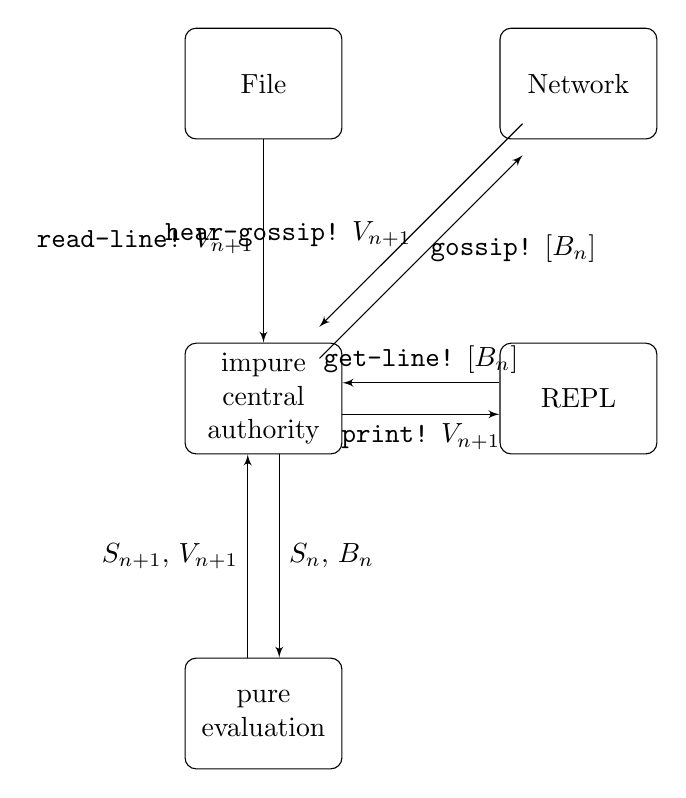
\begin{tikzpicture}[node distance = 4cm, auto]
  \node [block] (net) {Network};
  \node [block, below of=net] (repl) {REPL};
  \node [block, left of=repl] (impure) {impure central authority};
  \node [block, below of=impure] (pure) {pure evaluation};
  \node [block, above of=impure] (file) {File};

    \path [line]
    (file) -- node [left] {\texttt{read-line!} $V_{n+1}$} (impure);

    \path [line, transform canvas={yshift=0.2cm}]
    (net) -- node {\texttt{gossip!} [$B_n$]} (impure);
    \path [line, transform canvas={yshift=-0.2cm}]
    (impure) -- node {\texttt{hear-gossip!} $V_{n+1}$} (net);

    \path [line, transform canvas={yshift=0.2cm}]
    (repl) -- node [above] {\texttt{get-line!} [$B_n$]} (impure);
    \path [line, transform canvas={yshift=-0.2cm}]
    (impure) -- node [below] {\texttt{print!} $V_{n+1}$} (repl);

  \path [line, transform canvas={xshift=0.2cm}]
    (impure) -- node {$S_n$, $B_n$} (pure);
  \path [line, transform canvas={xshift=-0.2cm}]
    (pure) -- node {$S_{n+1}$, $V_{n+1}$} (impure);

\end{tikzpicture}
\caption{Effect system}
\label{f:effects}
\end{figure}

A further advantage of this approach is that, since on many blockchain
protocols new blocks have a low initial probability of being final (given the
possibility of forks), effects may be easily and programmatically delayed until
sufficiently many child blocks have been seen by simply buffering the
description of effects before passing them to the effect-handling layer.

\subsection{Data types} \rad's data types are: booleans (\texttt{\#t} and
\texttt{\#f}); strings (a sequence of characters within double quotes, with
\texttt{\textbackslash} as the escape character), symbols, lists, and numbers
(currently only arbitrary-precision decimals). These datatypes are all
immutable; additionally \rad supports \textit{refs} - mutable references - that
can hold any other datatype. Refs support a similar set of operations to
Clojure's atoms; however, they are not shareable across threads, and can be
interpreted as a pure state transformer.\footnote{The reference implementation
of \rad in fact uses Haskell's \texttt{STRef}s to implement refs, which in turn
use a by now well-known rank-2 type encapsulation to guarantee the property of
not being shareable across threads.\cite{lazy-functional-state-threads}}

\subsection{Syntax}


\subsection{Formal Semantics} We define the denotational semantics of \rad
recursively. The base case, $\mathcal{E}_{0}$, describes the denotation of a
term prior to any modification of \texttt{eval}. It's definition is given in
Figure \ref{f:denotationalsem0}.


\begin{figure}[H]
\begin{align*}
  \denotationdesc{0}{\variable}{\env \variable} \\
  \denotationdesc{0}{(\lam (\variable *) \rho^{+})}{} \\
  \denotationdesc{0}{(\define \variable \pi )}{} \\
  \denotationdesc{0}{(\deref \variable  )}{} \\
  \denotationdesc{0}{(\mkref \variable \pi)}{} \\
  \denotationdesc{0}{(\set \variable \pi)}{} \\
  \denotationdesc{0}{(\ifm \pi_0 \pi_1 \pi_2)}{}
\end{align*}
\caption{Denotational semantics for $\mathcal{E}_{0}$}
\label{f:denotationalsem0}
\end{figure}

After a redefinition of \texttt{eval}, the denotation of an expression is the
denotation of \texttt{eval} prior to the redefinition, applied to the
\textit{quoted} expression, as show in Figure \ref{f:denotationalsemn}.

\begin{figure}[H]
\begin{align*}
  \denotationdesc{n}{\pi}{(\denotation{n-1}{\evalm} (\quotem \pi))\rho}
\end{align*}
\caption{Denotational semantics for $\mathcal{E}_{n}$}
\label{f:denotationalsemn}
\end{figure}

Besides the forms described so far, additional forms exist which may be
implemented via \texttt{eval} redefinitions. They may also be implemented as
primitives; in either case, these forms must not be shadowable via
\texttt{define}s.

\section{Sample Programs and Chains}
\label{s:examples}


\bibliographystyle{plain}
\bibliography{bibliography,additional}
\end{multicols}


\appendix
\section{Syntax of \rad}

\setlength{\grammarindent}{5em}
\begin{figure}[H]
\begin{center}
\begin{grammar}
<expr> ::= <identifier>
\alt <literal>
\alt <application>
\alt <lambda>
\alt <define>
\alt <conditional>

<identifier> ::= <initial> <subsequent>*
\alt <special identifier>

<special identifier> ::= <special char>+

<special char> ::= `+' \alt `-' \alt <extended char>

<initial> ::= <letter> \alt <extended char>

<subsequent> ::= <letter> \alt <number> \alt <extended char>

<literal> ::= <boolean>
\alt <number>
\alt <string>

<boolean> ::= `#t' \alt `#f'

<string> ::= `"' <string element> `"'

<string element> ::= <any character other than `"' or `\'>
\alt `\\\"'
\alt `\\\\'

<comment> ::= `;;' <any character except newline> <newline>
\alt `#|' <character sequence not containing `|#'> `|#'

<application> ::= `(' <expr> <expr*> `)'

<conditional> ::= `(' `if' <expr> <expr> <expr> `)'


<define> ::= `(' `define' <identifier> <expr*> `)'
\end{grammar}
\end{center}
\caption{Syntax of \rad}
\end{figure}

\section{Derived Forms}

Derived forms are defined here as sample redefinitions of \texttt{eval}.


\subsection*{\texttt{quote}}

\begin{verbatim}
\end{verbatim}

\subsection*{\texttt{quasiquote}}

\begin{verbatim}
\end{verbatim}

\subsection*{\texttt{unquote}}

\begin{verbatim}
\end{verbatim}

\subsection*{\texttt{def}}

\begin{verbatim}

;; TODO: doc handling

(define eval (lambda (expr)
   (if (eq? (head expr) 'def)
       ((lambda ()
         (define pat (head (tail expr)))
         (define body (head (tail (tail expr))))
         (if (list? pat)
             (if (null? pat)
                 (error "def: bad name or pattern")
                 `(define ,(head pat) (lambda ,(tail pat) ,body)))
             `(define ,pat ,body))))
       expr))

\end{verbatim}

Example:

\begin{verbatim}
(def (factorial n)
  (:doc-str "The factorial function")
  (if (<= n 0)
      1
      (* n (factorial (- n 1))))

;; Which is equivalent to:

(begin
  (define factorial (lambda (n)
    (if (<= n 0)
        1
        (* n (factorial (- n 1)))))
  (add-doc-str factorial "The factorial function")
\end{verbatim}

\end{document}
